% Use xelatex to generate a pdf file of this presentation

\documentclass{beamer}
\usepackage{roboto}
\usepackage[english]{babel}
\usetheme{Copenhagen}

% Simple way to put a code listing to the slide
\usepackage{listings}

\usepackage{tikz}
\usetikzlibrary{positioning}
\usepackage{pgfplots}
\pgfplotsset{compat=1.18}
\usepackage{graphicx}
\usepackage{qrcode}
\usepackage{booktabs}

% Blocks settings
\setbeamerfont{block title}{size=\tiny}
\setbeamertemplate{navigation symbols}{}

%Information to be included in the title page:
\title{Multi-Insert in Logical Replication}
\subtitle{Batching the Apply Worker for Fun and Throughput}
\author{Andrei Lepikhov}
\institute{pgEdge}
\date{09.05.2026}

% Add page numbers in the footnote
\expandafter\def\expandafter\insertshorttitle\expandafter{%
  \insertshorttitle\hfill%
  \insertframenumber\,/\,\inserttotalframenumber}

\definecolor{lightlightgray}{gray}{0.9}
\definecolor{pgblue}{HTML}{336791}
\definecolor{pgorange}{HTML}{E8781A}

% Default listing format
\lstset{language=sql, frame=none, tabsize=2, identifierstyle=\color{black},
  showspaces=false, showtabs=false, showstringspaces=false,
  columns=fullflexible, % Restore default spaces between letters
  basicstyle=\rmfamily\scriptsize,
  stringstyle=\color{purple},
  keywordstyle=\bfseries\color{green!40!black},
  numberstyle=\tiny\color{gray},
  morekeywords={PUBLICATION,SUBSCRIPTION,CONNECTION,WITH,COPY,FORMAT}}

% -----------------------------

\begin{document}

% %%%%%%%%%%%%%%%%%%%%%%%%%%%%%%%%%%%%%%%%%%%%%%%%%%%%%%%%%%%%%%%%%%%%%%%%
% Title
% %%%%%%%%%%%%%%%%%%%%%%%%%%%%%%%%%%%%%%%%%%%%%%%%%%%%%%%%%%%%%%%%%%%%%%%%

\begin{frame}
\titlepage
\end{frame}

% %%%%%%%%%%%%%%%%%%%%%%%%%%%%%%%%%%%%%%%%%%%%%%%%%%%%%%%%%%%%%%%%%%%%%%%%
% Why This Matters
% %%%%%%%%%%%%%%%%%%%%%%%%%%%%%%%%%%%%%%%%%%%%%%%%%%%%%%%%%%%%%%%%%%%%%%%%

\begin{frame}
\vspace*{\fill}\begin{center}
\huge{Why This Matters}
\end{center}\vspace*{\fill}
\end{frame}

\begin{frame}\frametitle{Motivation}
\textbf{1. Async replication needs minimal lag.}\\
Logical replication is asynchronous --- every second of apply delay
is a second of data you cannot read on the subscriber.
Reducing per-tuple overhead shrinks that window.

\bigskip
\textbf{2. Bulk influx is the typical pattern.}\\
End-of-month batch loads, nightly ETL jobs ---
real workloads frequently arrive in bursts, not drips.
The apply worker must handle millions of INSERTs at wire speed.

\bigskip
\textbf{3. Multi-region means low-bandwidth channels.}\\
Multi-cloud and cross-continent logical replication runs over
constrained links. Every extra byte of WAL on the subscriber is
wasted disk I/O \textit{and} wasted recovery time when the link catches up.

\bigskip
{\small\textit{Today the subscriber can write significantly more WAL than the publisher
for the same COPY --- pure overhead.}}
\end{frame}

% The most important part is potential specialisation of the Spock on multi-region loads that might need more sophisticated tools to reduce network consumption.

% %%%%%%%%%%%%%%%%%%%%%%%%%%%%%%%%%%%%%%%%%%%%%%%%%%%%%%%%%%%%%%%%%%%%%%%%
% The Problem
% %%%%%%%%%%%%%%%%%%%%%%%%%%%%%%%%%%%%%%%%%%%%%%%%%%%%%%%%%%%%%%%%%%%%%%%%

\begin{frame}
\vspace*{\fill}\begin{center}
\huge{The Problem}
\end{center}\vspace*{\fill}
\end{frame}

\begin{frame}[fragile]\frametitle{How COPY Loads Data on the Publisher}
\begin{center}
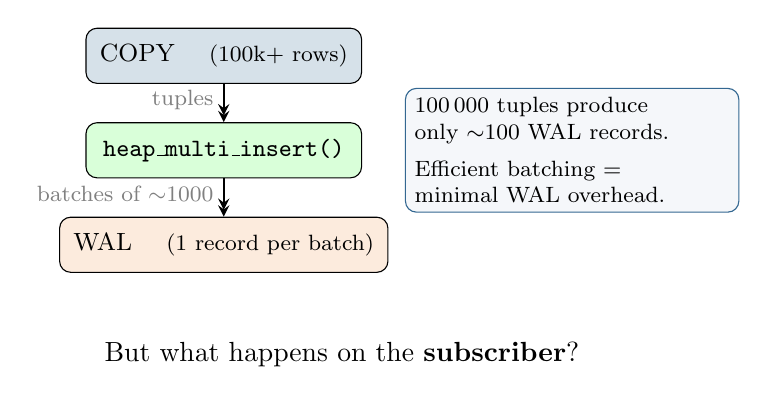
\begin{tikzpicture}[
  box/.style={draw, rounded corners, minimum height=0.7cm,
              align=center, font=\small, inner sep=5pt},
  arr/.style={->, thick, >=stealth},
  lbl/.style={font=\footnotesize, text=gray},
]

% ---- Vertical pipeline (shifted left) ----
\node[box, fill=pgblue!20, minimum width=3.5cm] (copy) at (-1.5, 0)
  {COPY \quad {\footnotesize(100k+ rows)}};

\draw[arr] (copy.south) -- ++(0, -0.4)
  node[midway, left, lbl] {tuples} coordinate (m1);

\node[box, fill=green!15, minimum width=3.5cm] (hmi) at (-1.5, -1.2)
  {\texttt{heap\_multi\_insert()}};

\draw[arr] (m1) -- (hmi.north);

\draw[arr] (hmi.south) -- ++(0, -0.4)
  node[midway, left, lbl] {batches of $\sim$1000} coordinate (m2);

\node[box, fill=pgorange!15, minimum width=3.5cm] (wal) at (-1.5, -2.4)
  {WAL \quad {\footnotesize(1 record per batch)}};

\draw[arr] (m2) -- (wal.north);

% ---- Key insight (right side, well separated) ----
\node[draw=pgblue, rounded corners, fill=pgblue!5,
      font=\footnotesize, align=left, text width=4cm,
      anchor=west] at (0.8, -1.2)
  {100\,000 tuples produce\\
   only $\sim$100 WAL records.\\[4pt]
   Efficient batching =\\
   minimal WAL overhead.};

% ---- Teaser ----
\node[font=\normalsize, align=center] at (0, -3.8)
  {But what happens on the \textbf{subscriber}?};

\end{tikzpicture}
\end{center}
\end{frame}

\begin{frame}[fragile]\frametitle{Without Batching, Subscriber WAL Exceeds Publisher}
\begin{center}
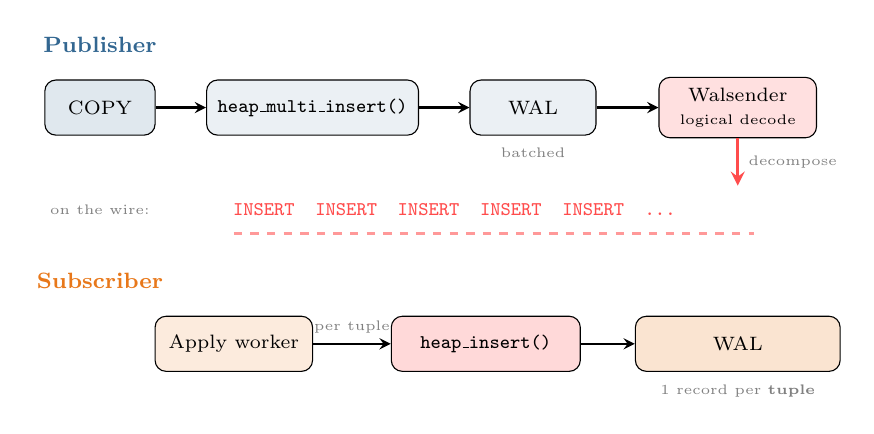
\begin{tikzpicture}[
  box/.style={draw, rounded corners, minimum height=0.7cm,
              align=center, font=\scriptsize, inner sep=4pt},
  arr/.style={->, thick, >=stealth},
  lbl/.style={font=\tiny, text=gray},
  phase/.style={font=\footnotesize\bfseries},
]
% ---- Row 1: Publisher pipeline (left to right) ----
\node[phase, text=pgblue] at (-4.5, 0.8) {Publisher};

\node[box, fill=pgblue!15, minimum width=1.4cm] (cpy) at (-4.5, 0) {COPY};
\node[box, fill=pgblue!10, minimum width=2.6cm] (multi) at (-1.8, 0)
  {\texttt{heap\_multi\_insert()}};
\node[box, fill=pgblue!10, minimum width=1.6cm] (wal) at (1.0, 0)
  {WAL};
\node[box, fill=red!12, minimum width=2.0cm] (decode) at (3.6, 0)
  {Walsender\\{\tiny logical decode}};

\draw[arr] (cpy) -- (multi);
\draw[arr] (multi) -- (wal);
\draw[arr] (wal) -- (decode);

\node[lbl, below=1pt of wal] {batched};

% ---- Arrow down: decomposition ----
\draw[arr, red!70, very thick] (decode.south) -- ++(0,-0.6)
  node[right, lbl, pos=0.5] {decompose}
  coordinate (mid);

% ---- Row 2: Network ----
\node[lbl] at (-4.5, -1.3) {on the wire:};
\node[font=\scriptsize\ttfamily, text=red!70] at (0, -1.3)
  {INSERT\ \ INSERT\ \ INSERT\ \ INSERT\ \ INSERT\ \ \ldots};
\draw[dashed, red!40, thick] (-2.8, -1.6) -- (3.8, -1.6);

% ---- Row 3: Subscriber pipeline (left to right) ----
\node[phase, text=pgorange] at (-4.5, -2.2) {Subscriber};

\node[box, fill=pgorange!15, minimum width=2.0cm] (apply) at (-2.8, -3.0)
  {Apply worker};
\node[box, fill=red!15, minimum width=2.4cm] (hi) at (0.4, -3.0)
  {\texttt{heap\_insert()}};
\node[box, fill=pgorange!20, minimum width=2.6cm] (swal) at (3.6, -3.0)
  {WAL};

\draw[arr] (apply) -- node[above, lbl] {per tuple} (hi);
\draw[arr] (hi) -- (swal);

\node[lbl, below=1pt of swal] {1 record per \textbf{tuple}};

\end{tikzpicture}
\end{center}
\begin{alertblock}{}
\centering
\small Publisher COPY writes 13\,GB of WAL $\Rightarrow$ subscriber generates
\textbf{$\sim$18\,GB}.\\[1pt]
WAL amplification on subscriber. Slow catch-up. Wasted I/O.
\end{alertblock}
\end{frame}

% %%%%%%%%%%%%%%%%%%%%%%%%%%%%%%%%%%%%%%%%%%%%%%%%%%%%%%%%%%%%%%%%%%%%%%%%
% The Idea
% %%%%%%%%%%%%%%%%%%%%%%%%%%%%%%%%%%%%%%%%%%%%%%%%%%%%%%%%%%%%%%%%%%%%%%%%

\begin{frame}[fragile]\frametitle{The Fix: Batch Inserts in the Apply Worker}
\begin{center}
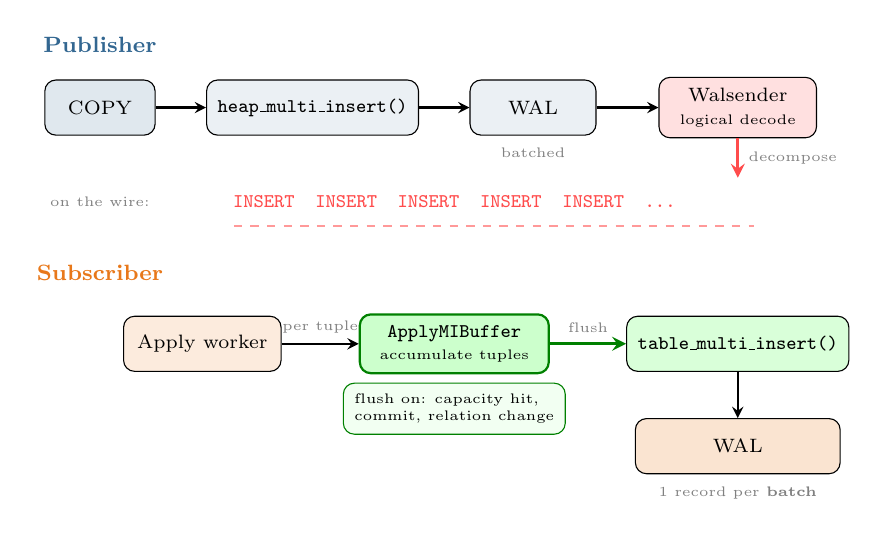
\begin{tikzpicture}[
  box/.style={draw, rounded corners, minimum height=0.7cm,
              align=center, font=\scriptsize, inner sep=4pt},
  arr/.style={->, thick, >=stealth},
  lbl/.style={font=\tiny, text=gray},
  phase/.style={font=\footnotesize\bfseries},
]
% ---- Row 1: same Publisher pipeline as before ----
\node[phase, text=pgblue] at (-4.5, 0.8) {Publisher};

\node[box, fill=pgblue!15, minimum width=1.4cm] (cpy) at (-4.5, 0) {COPY};
\node[box, fill=pgblue!10, minimum width=2.6cm] (multi) at (-1.8, 0)
  {\texttt{heap\_multi\_insert()}};
\node[box, fill=pgblue!10, minimum width=1.6cm] (wal) at (1.0, 0) {WAL};
\node[box, fill=red!12, minimum width=2.0cm] (decode) at (3.6, 0)
  {Walsender\\{\tiny logical decode}};

\draw[arr] (cpy) -- (multi);
\draw[arr] (multi) -- (wal);
\draw[arr] (wal) -- (decode);
\node[lbl, below=1pt of wal] {batched};

% ---- Network ----
\draw[arr, red!70, very thick] (decode.south) -- ++(0,-0.5)
  node[right, lbl, pos=0.5] {decompose} coordinate (mid);
\node[lbl] at (-4.5, -1.2) {on the wire:};
\node[font=\scriptsize\ttfamily, text=red!70] at (0, -1.2)
  {INSERT\ \ INSERT\ \ INSERT\ \ INSERT\ \ INSERT\ \ \ldots};
\draw[dashed, red!40, thick] (-2.8, -1.5) -- (3.8, -1.5);

% ---- Row 2: NEW Subscriber pipeline ----
\node[phase, text=pgorange] at (-4.5, -2.1) {Subscriber};

\node[box, fill=pgorange!15, minimum width=2.0cm] (apply) at (-3.2, -3.0)
  {Apply worker};
\node[box, fill=green!20, minimum width=2.4cm, thick,
      draw=green!50!black] (buf) at (0.0, -3.0)
  {\texttt{ApplyMIBuffer}\\{\tiny accumulate tuples}};
\node[box, fill=green!15, minimum width=2.6cm] (tmi) at (3.6, -3.0)
  {\texttt{table\_multi\_insert()}};

\draw[arr] (apply) -- node[above, lbl] {per tuple} (buf);
\draw[arr, green!50!black, very thick] (buf) -- node[above, lbl] {flush} (tmi);

% ---- WAL output (below) ----
\node[box, fill=pgorange!20, minimum width=2.6cm] (swal) at (3.6, -4.3)
  {WAL};
\draw[arr] (tmi) -- (swal);
\node[lbl, below=1pt of swal] {1 record per \textbf{batch}};

% ---- Flush triggers annotation ----
\node[draw=green!50!black, rounded corners, fill=green!5,
      font=\tiny, align=left, inner sep=4pt,
      below=3pt of buf] (triggers)
  {flush on: capacity hit,\\
   commit, relation change};

\end{tikzpicture}
\end{center}
\end{frame}

\begin{frame}\frametitle{Why No MULTI\_INSERT in the community Protocol?}
\bigskip

\begin{itemize}\setlength{\itemsep}{8pt}
  \item \textbf{Not a SQL operation.}\\
        Protocol mirrors SQL changes; \texttt{heap\_multi\_insert()} is
        internal to COPY.
  \item \textbf{Protocol version negotiation.}\\
        New message type $\Rightarrow$ version bump, fallback paths,
        coordination cost.
  \item \textbf{Conflict resolution becomes harder.}\\
        Batch is all-or-nothing --- must unpack and retry row-by-row
        on conflict.
  \item \textbf{Output plugin API is per-change.}\\
        \texttt{LogicalDecodeChangeCB} receives one change ---
        batch API breaks all existing plugins.
\end{itemize}
\end{frame}

\begin{frame}[fragile]\frametitle{Enabling Multi-Insert}
\begin{lstlisting}
-- Automatic slot creation:
CREATE SUBSCRIPTION mysub
  CONNECTION 'host=publisher port=5432 dbname=mydb'
  PUBLICATION mypub
  WITH (multi_insert = on, streaming = off);
\end{lstlisting}
\bigskip
\begin{lstlisting}
-- With a manually created slot:
-- 1. On publisher (replication connection):
CREATE_REPLICATION_SLOT mysub_slot LOGICAL pgoutput;

-- 2. On subscriber:
CREATE SUBSCRIPTION mysub
  CONNECTION 'host=publisher port=5432 dbname=mydb'
  PUBLICATION mypub
  WITH (
    create_slot = false,
    slot_name = 'mysub_slot',
    multi_insert = on,
    streaming = off
  );
\end{lstlisting}
\smallskip
{\small \texttt{multi\_insert} is always a subscription option ---
no protocol changes.}
\end{frame}

% %%%%%%%%%%%%%%%%%%%%%%%%%%%%%%%%%%%%%%%%%%%%%%%%%%%%%%%%%%%%%%%%%%%%%%%%
% Implementation
% %%%%%%%%%%%%%%%%%%%%%%%%%%%%%%%%%%%%%%%%%%%%%%%%%%%%%%%%%%%%%%%%%%%%%%%%

\begin{frame}
\vspace*{\fill}\begin{center}
\huge{Implementation}
\end{center}\vspace*{\fill}
\end{frame}

\begin{frame}[fragile]\frametitle{ApplyMIBuffer --- The Batching Engine}
\begin{columns}[T]
\begin{column}{0.55\textwidth}
\textbf{Lifecycle:}
\begin{enumerate}
  \item Single static buffer, initialized on first
        INSERT for an eligible relation
  \item Accumulate tuples in slot array
  \item \textbf{Intermediate flush:} capacity hit $\to$ call
        \texttt{table\_multi\_insert()}, clear slots, reuse buffer
  \item \textbf{Final flush:} commit, relation change,
        or non-INSERT event $\to$ flush and reinitialize
        for the next relation
\end{enumerate}
\end{column}
\begin{column}{0.4\textwidth}
\textbf{Slot management:}
\begin{itemize}
  \item Fixed array of 10\,000 \texttt{TupleTableSlot*},
        lazily allocated one per tuple
  \item Slots reused across flushes (only \texttt{nslots} resets to 0)
  \item Flush when \texttt{nslots} $\geq$ 10\,000
        or \texttt{cum\_bytes} $\geq$ 8\,MB
\end{itemize}
\end{column}
\end{columns}
\end{frame}

% Eligibility rules verified against apply_mi_relation_is_safe() at b971fed6d80.
%
% Why each restriction exists (LR bypasses the executor pipeline that
% COPY uses, so constraints must be checked statically):
%
%   Triggers (any):    COPY only rejects BEFORE ROW / INSTEAD OF.
%                      LR rejects ALL triggers because apply_handle_insert()
%                      fires triggers outside the batch path --- mixing the
%                      two would double-fire or skip triggers.
%
%   RLS:               Policies may filter/reject rows.  COPY does NOT
%                      restrict on RLS (it runs through the executor).
%                      LR skips the executor, so RLS is unchecked.
%
%   CHECK constraints: Can raise per-tuple errors.  COPY does NOT restrict
%                      (checks happen via the executor).  LR inserts
%                      directly via table_multi_insert(), skipping checks.
%
%   Stored generated:  Need per-tuple expression evaluation.  Same as CHECK.
%
%   Exclusion constr:  Cannot be validated with table_multi_insert() ---
%                      would need per-tuple ExecInsertIndexTuples.
%
%   Deferrable UNIQUE: Conflict cannot be detected at insert time;
%                      deferred check at commit may find batch-internal
%                      duplicates.  Immediate UNIQUE/PK is allowed.
%
%   Invalid/unready    Indexes in a broken state --- inserting into them
%   indexes:           would corrupt the index or silently skip entries.
%
%   Non-plain table:   Partitioned tables, foreign tables, views excluded.
%                      AM must provide multi_insert callback.
%
% COPY has restrictions that LR does not:
%   - Volatile default expressions (LR evaluates defaults before buffering)
%   - Volatile WHERE clause (N/A in LR context)
%   - Foreign tables without FDW batching support (excluded by relkind in LR)
%
\begin{frame}\frametitle{Not Every Table Qualifies for Batching}
A table is eligible for multi-insert if it has \textbf{none} of:
\bigskip

\begin{columns}[T]
\begin{column}{0.45\textwidth}
\begin{itemize}
  \item BEFORE/INSTEAD OF triggers
  \item \textit{Row-level security}
  \item \textit{CHECK constraints}
  \item \textit{Stored generated columns}
\end{itemize}
\end{column}
\begin{column}{0.45\textwidth}
\begin{itemize}
  \item \textit{Exclusion constraints}
  \item \textit{Deferrable UNIQUE/PK}
  \item \textit{Invalid or unready indexes}
  \item Non-plain table (partitioned, foreign)
\end{itemize}
\end{column}
\end{columns}
\bigskip
Ineligible tables \textbf{silently fall back} to per-tuple insert.

\smallskip
{Stricter than COPY: LR bypasses the executor,
so constraints that COPY validates at runtime must be rejected statically.}
\end{frame}


% %%%%%%%%%%%%%%%%%%%%%%%%%%%%%%%%%%%%%%%%%%%%%%%%%%%%%%%%%%%%%%%%%%%%%%%%
% Benchmarks
% %%%%%%%%%%%%%%%%%%%%%%%%%%%%%%%%%%%%%%%%%%%%%%%%%%%%%%%%%%%%%%%%%%%%%%%%

\begin{frame}\frametitle{Benchmark Setup}
\begin{center}
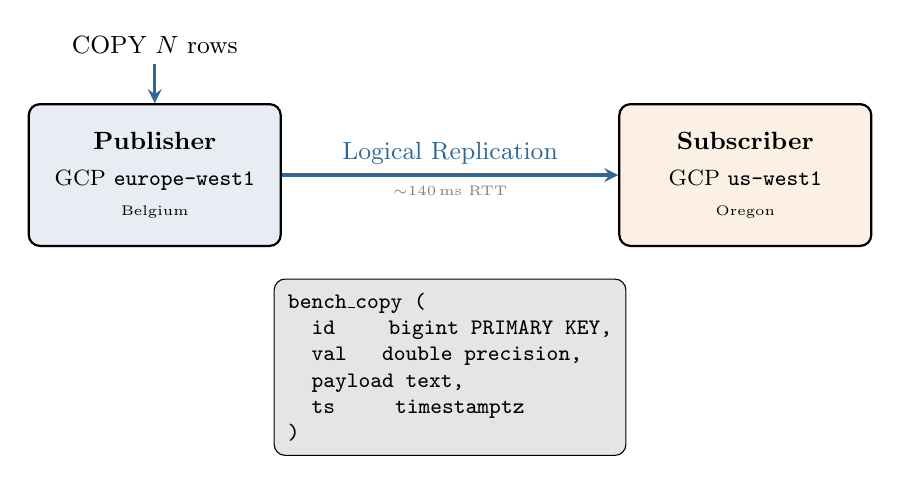
\begin{tikzpicture}[
  vm/.style={draw, rounded corners, minimum width=3.2cm, minimum height=1.8cm,
             align=center, font=\small, thick},
  lbl/.style={font=\tiny\ttfamily, text=gray},
  arr/.style={->, very thick, >=stealth, pgblue},
]
% Publisher
\node[vm, fill=pgblue!12] (pub) at (0,0) {
  \textbf{Publisher}\\[2pt]
  {\footnotesize GCP \texttt{europe-west1}}\\
  {\tiny Belgium}
};
% Subscriber
\node[vm, fill=pgorange!12] (sub) at (7.5,0) {
  \textbf{Subscriber}\\[2pt]
  {\footnotesize GCP \texttt{us-west1}}\\
  {\tiny Oregon}
};
% Arrow
\draw[arr] (pub) -- node[above, font=\small] {Logical Replication}
                     node[below, font=\tiny, text=gray] {$\sim$140\,ms RTT}
           (sub);
% COPY arrow into publisher
\node[font=\small, above=0.5cm of pub] (copy) {COPY $N$ rows};
\draw[arr] (copy) -- (pub);
% Table schema below
\node[below=0.4cm of pub, xshift=3.75cm, draw, rounded corners,
      fill=lightlightgray, inner sep=5pt, font=\footnotesize\ttfamily,
      align=left] (schema) {
  bench\_copy (\\
  \quad id \quad\; bigint PRIMARY KEY,\\
  \quad val \quad double precision,\\
  \quad payload text,\\
  \quad ts \quad\;\; timestamptz\\
  )
};
\end{tikzpicture}
\end{center}
\vspace{-4mm}
\begin{itemize}\small
  \item Three dataset sizes: 1M, 10M, 100M rows
  \item \texttt{multi\_insert = true} vs \texttt{false}, \texttt{streaming = off}
\end{itemize}
\end{frame}

\begin{frame}\frametitle{Multi-insert halves replication catch-up}
\begin{center}
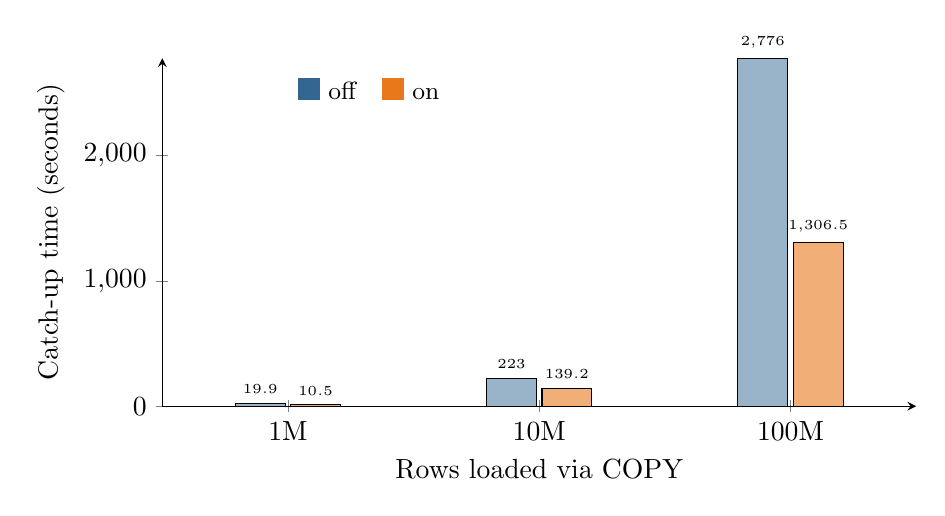
\begin{tikzpicture}
\begin{axis}[
    ybar,
    bar width=18pt,
    width=0.92\textwidth,
    height=6cm,
    ylabel={Catch-up time (seconds)},
    symbolic x coords={1M,10M,100M},
    xtick=data,
    xlabel={Rows loaded via COPY},
    ymin=0,
    axis x line=bottom,
    axis y line=left,
    nodes near coords,
    nodes near coords style={font=\tiny, above},
    enlarge x limits=0.25,
]
\addplot[fill=pgblue!50] coordinates {(1M,19.9) (10M,223.0) (100M,2776.0)};
\addplot[fill=pgorange!60] coordinates {(1M,10.5) (10M,139.2) (100M,1306.5)};
% Direct labels — top-left annotation
\node[font=\small, anchor=north west, align=left] at (axis cs:1M,2700)
  {{\color{pgblue}\rule{8pt}{8pt}} off\quad
   {\color{pgorange}\rule{8pt}{8pt}} on};
\end{axis}
\end{tikzpicture}
\end{center}
\begin{center}
\textbf{1.6$\times$ -- 2.1$\times$ faster} replication catch-up across all sizes.
\end{center}
\end{frame}

\begin{frame}\frametitle{Multi-insert cuts subscriber WAL by 19--28\%}
\begin{center}
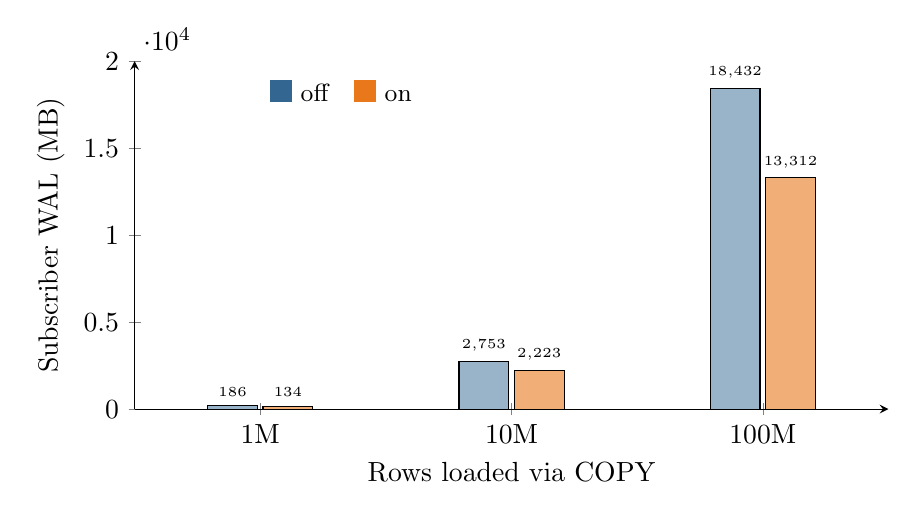
\begin{tikzpicture}
\begin{axis}[
    ybar,
    bar width=18pt,
    width=0.92\textwidth,
    height=6cm,
    ylabel={Subscriber WAL (MB)},
    symbolic x coords={1M,10M,100M},
    xtick=data,
    xlabel={Rows loaded via COPY},
    ymin=0,
    ymax=20000,
    axis x line=bottom,
    axis y line=left,
    nodes near coords,
    nodes near coords style={font=\tiny, above},
    enlarge x limits=0.25,
]
\addplot[fill=pgblue!50] coordinates {(1M,186) (10M,2753) (100M,18432)};
\addplot[fill=pgorange!60] coordinates {(1M,134) (10M,2223) (100M,13312)};
% Direct labels — top-left annotation
\node[font=\small, anchor=north west, align=left] at (axis cs:1M,19500)
  {{\color{pgblue}\rule{8pt}{8pt}} off\quad
   {\color{pgorange}\rule{8pt}{8pt}} on};
\end{axis}
\end{tikzpicture}
\end{center}
\begin{center}
At 100M rows: 18\,GB $\to$ 13\,GB.
\end{center}
\end{frame}

\begin{frame}\frametitle{The Numbers at a Glance}
\begin{center}
\begin{tabular}{l rr rr}
  \toprule
  & \multicolumn{2}{c}{\textbf{Catch-up (s)}}
  & \multicolumn{2}{c}{\textbf{Subscriber WAL}} \\
  \cmidrule(lr){2-3}\cmidrule(lr){4-5}
  \textbf{Rows} & off & on & off & on \\
  \midrule
  1M   & 19.9   & 10.5   & 186\,MB  & 134\,MB \\
  10M  & 223.0  & 139.2  & 2.7\,GB  & 2.2\,GB \\
  100M & 2\,776 & 1\,307 & 18\,GB   & 13\,GB  \\
  \midrule
  \textbf{Speedup} & \multicolumn{2}{c}{\textbf{1.6--2.1$\times$}}
                    & \multicolumn{2}{c}{\textbf{$-$19\% to $-$28\%}} \\
  \bottomrule
\end{tabular}
\end{center}
\bigskip
Publisher COPY time and publisher WAL are \textbf{unchanged} ---
the optimisation is purely subscriber-side.
\end{frame}

% %%%%%%%%%%%%%%%%%%%%%%%%%%%%%%%%%%%%%%%%%%%%%%%%%%%%%%%%%%%%%%%%%%%%%%%%
% Challenges
% %%%%%%%%%%%%%%%%%%%%%%%%%%%%%%%%%%%%%%%%%%%%%%%%%%%%%%%%%%%%%%%%%%%%%%%%

\begin{frame}\frametitle{Current Limitations and Open Problems}
\begin{itemize}
  \item \textbf{Conflicts and errors cause fallback to single-insert.}\\
        {\small A unique violation or other error during batch flush aborts
        the remote transaction. Standard per-row conflict resolution
        (\texttt{disable\_on\_error}, \texttt{SKIP}) is bypassed.}
  \medskip
  \item \textbf{Streaming must incorporate batching.}\\
        {\small Currently \texttt{multi\_insert} requires
        \texttt{streaming = off}. Combining both is needed for
        a production-ready version.}
  \medskip
  \item \textbf{Parallel apply workers excluded.}\\
        {\small Multi-insert is disabled inside parallel apply workers.}
  \medskip
  \item \textbf{Per-transaction disable on first ineligible relation.}\\
        {\small If any relation fails the eligibility check, batching is
        disabled for the \emph{entire} remaining transaction, even for
        other eligible tables.}
\end{itemize}
\end{frame}

% %%%%%%%%%%%%%%%%%%%%%%%%%%%%%%%%%%%%%%%%%%%%%%%%%%%%%%%%%%%%%%%%%%%%%%%%
% Future Work
% %%%%%%%%%%%%%%%%%%%%%%%%%%%%%%%%%%%%%%%%%%%%%%%%%%%%%%%%%%%%%%%%%%%%%%%%

\begin{frame}\frametitle{Future: publisher-side batching}
\begin{center}
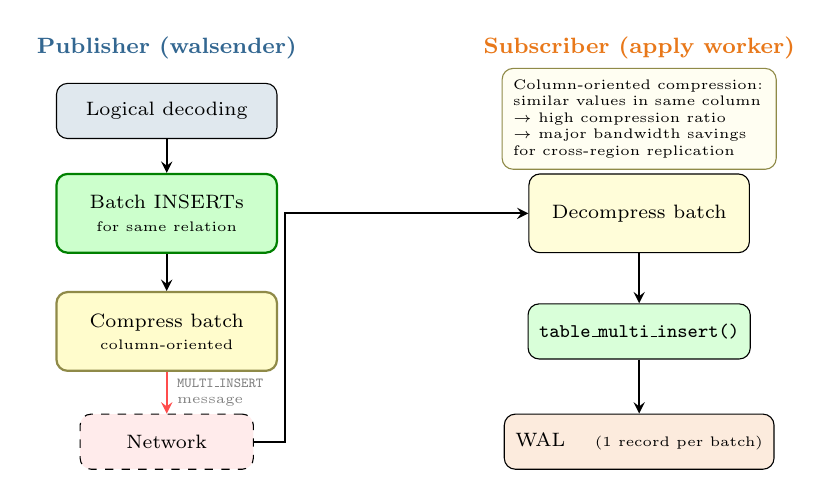
\begin{tikzpicture}[
  box/.style={draw, rounded corners, minimum height=0.7cm,
              align=center, font=\scriptsize, inner sep=4pt},
  arr/.style={->, thick, >=stealth},
  lbl/.style={font=\tiny, text=gray},
  phase/.style={font=\footnotesize\bfseries},
]

% ---- Publisher ----
\node[phase, text=pgblue] at (-1.5, 1.6) {Publisher (walsender)};

\node[box, fill=pgblue!15, minimum width=2.8cm] (decode) at (-1.5, 0.8)
  {Logical decoding};

\node[box, fill=green!20, thick, draw=green!50!black,
      minimum width=2.8cm, minimum height=1.0cm] (batch) at (-1.5, -0.5)
  {Batch INSERTs\\{\tiny for same relation}};

\node[box, fill=yellow!20, thick, draw=yellow!50!black,
      minimum width=2.8cm, minimum height=1.0cm] (compress) at (-1.5, -2.0)
  {Compress batch\\{\tiny column-oriented}};

\draw[arr] (decode) -- (batch);
\draw[arr] (batch) -- (compress);

% ---- Wire ----
\node[box, fill=red!8, dashed, minimum width=2.2cm] (wire) at (-1.5, -3.4)
  {Network};
\draw[arr, red!70] (compress) -- node[right, lbl, align=left]
  {\texttt{MULTI\_INSERT}\\message} (wire);

% ---- Subscriber ----
\node[phase, text=pgorange] at (4.5, 1.6) {Subscriber (apply worker)};

\node[box, fill=yellow!15, minimum width=2.8cm, minimum height=1.0cm]
  (decomp) at (4.5, -0.5)
  {Decompress batch};

\node[box, fill=green!15, minimum width=2.8cm] (tmi) at (4.5, -2.0)
  {\texttt{table\_multi\_insert()}};

\node[box, fill=pgorange!15, minimum width=2.8cm] (wal) at (4.5, -3.4)
  {WAL \quad {\tiny(1 record per batch)}};

\draw[arr] (wire.east) -- ++(0.4, 0) |- (decomp.west);
\draw[arr] (decomp) -- (tmi);
\draw[arr] (tmi) -- (wal);

% ---- Annotation: compression ----
\node[draw=yellow!50!black, rounded corners, fill=yellow!5,
      font=\tiny, align=left, inner sep=4pt, text width=3.2cm]
  at (4.5, 0.7) (note)
  {Column-oriented compression:\\
   similar values in same column\\
   $\to$ high compression ratio\\
   $\to$ major bandwidth savings\\
   for cross-region replication};

\end{tikzpicture}
\end{center}
\end{frame}

% %%%%%%%%%%%%%%%%%%%%%%%%%%%%%%%%%%%%%%%%%%%%%%%%%%%%%%%%%%%%%%%%%%%%%%%%
% Closing
% %%%%%%%%%%%%%%%%%%%%%%%%%%%%%%%%%%%%%%%%%%%%%%%%%%%%%%%%%%%%%%%%%%%%%%%%

\begin{frame}\frametitle{Summary}
\begin{itemize}
  \item Logical replication apply worker now supports batched inserts
  \item \textbf{2$\times$ faster} replication catch-up on bulk loads
  \item \textbf{28\% less WAL} generated on the subscriber
  \item Subscriber-side only --- zero publisher changes
  \item Opt-in via \texttt{multi\_insert = on}, graceful fallback
\end{itemize}
\bigskip
\begin{center}
\begin{columns}[c]
\begin{column}{0.45\textwidth}
\centering
\qrcode[height=2.2cm]{https://github.com/danolivo/pgdev/tree/lr-multi-insert}
\vspace{2mm}\\
{\tiny Code}
\end{column}
\begin{column}{0.45\textwidth}
\centering
\qrcode[height=2.2cm]{https://github.com/danolivo/conf/tree/main/2026c-LR-Multi-Insert}
\vspace{2mm}\\
{\tiny Benchmarks \& materials}
\end{column}
\end{columns}
\end{center}
\end{frame}
\begin{frame}
\vspace*{\fill}
\begin{center}
\huge{Questions?}
\bigskip

\end{center}
\vspace*{\fill}
\end{frame}


\begin{frame}\frametitle{Publisher Side: Many Writers, Few Senders, One WAL}
\begin{center}
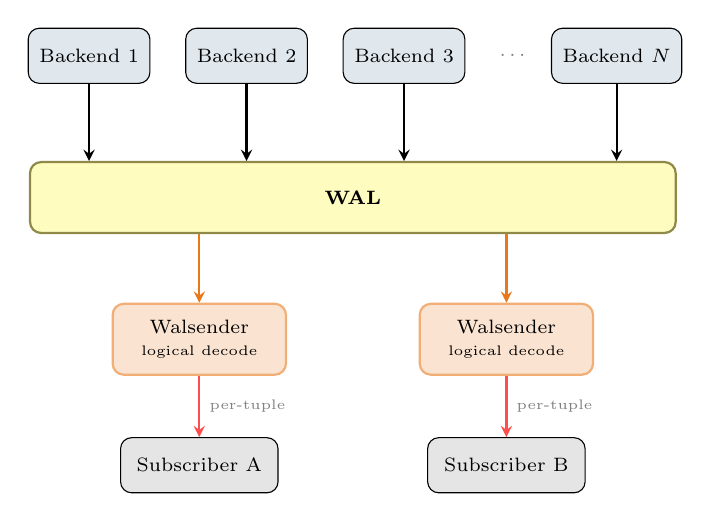
\begin{tikzpicture}[
  box/.style={draw, rounded corners, minimum height=0.7cm,
              align=center, font=\scriptsize, inner sep=4pt},
  arr/.style={->, thick, >=stealth},
  lbl/.style={font=\tiny, text=gray},
  phase/.style={font=\footnotesize\bfseries},
]

% ---- Backends ----
\node[box, fill=pgblue!15, minimum width=1.4cm] (b1) at (-3.2, 1.8) {Backend 1};
\node[box, fill=pgblue!15, minimum width=1.4cm] (b2) at (-1.2, 1.8) {Backend 2};
\node[box, fill=pgblue!15, minimum width=1.4cm] (b3) at (0.8, 1.8)  {Backend 3};
\node[font=\scriptsize, text=gray] at (2.2, 1.8) {\ldots};
\node[box, fill=pgblue!15, minimum width=1.4cm] (bn) at (3.5, 1.8)  {Backend $N$};

% ---- WAL ----
\node[box, fill=yellow!25, minimum width=8.2cm, minimum height=0.9cm,
      thick, draw=yellow!50!black] (wal) at (0.15, 0)
  {\textbf{WAL}};

\draw[arr] (b1.south) -- (wal.north -| b1.south);
\draw[arr] (b2.south) -- (wal.north -| b2.south);
\draw[arr] (b3.south) -- (wal.north -| b3.south);
\draw[arr] (bn.south) -- (wal.north -| bn.south);

% ---- Walsenders ----
\node[box, fill=pgorange!20, minimum width=2.2cm, minimum height=0.9cm,
      thick, draw=pgorange!60] (ws1) at (-1.8, -1.8)
  {Walsender\\{\tiny logical decode}};
\node[box, fill=pgorange!20, minimum width=2.2cm, minimum height=0.9cm,
      thick, draw=pgorange!60] (ws2) at (2.1, -1.8)
  {Walsender\\{\tiny logical decode}};

\draw[arr, pgorange] (wal.south -| ws1.north) -- (ws1.north);
\draw[arr, pgorange] (wal.south -| ws2.north) -- (ws2.north);

% ---- Subscribers ----
\node[box, fill=lightlightgray, minimum width=2.0cm] (sub1) at (-1.8, -3.4)
  {Subscriber A};
\node[box, fill=lightlightgray, minimum width=2.0cm] (sub2) at (2.1, -3.4)
  {Subscriber B};

\draw[arr, red!70] (ws1) -- node[right, lbl] {per-tuple} (sub1);
\draw[arr, red!70] (ws2) -- node[right, lbl] {per-tuple} (sub2);

\end{tikzpicture}
\end{center}
\end{frame}


\end{document}
